\chapter{Evaluación del modelo}
\label{chap:evaluacion}
Recordemos que el problema que buscamos resolver a través de este modelo es el de priorizar correctamente las verificaciones domiciliarias, reduciendo así la proporción de hogares que son sujetos a un proceso de focalización incorrecta. Dada la deriva temporal a la que está sujeto el proceso de focalización -los programas que operan en cierta región, así como los criterios que utilizan para focalizar, están cambiando constantemente- simplificamos el problema al definir que nuestro objetivo es, simplemente, asignar correctamente las verificaciones. Definimos como una verificación correctamente asignada a aquella en la que se tuvo que corregir el valor de al menos una variable. Así, podemos utilizar la distribución posterior resultante de nuestro modelo bayesiano para definir un clasificador que indique una verificación a realizar en caso de que haya una probabilidad de tener cambios suficientemente alta.
\par
\noindent
Podemos entonces comparar entre conjuntos de variables como comparamos entre clasificadores. Sin embargo, dado un conjunto de variables, necesitamos escoger el valor de $k$ que resulte en la estructura más adecuada. Definimos entonces nuestro proceso de evaluación de modelos en dos pasos.
\section*{Comparación de estructuras}
Lo primero que necesitamos asegurar es que, dado un conjunto de variables, tenemos la mejor estructura posible que el algoritmo sea capaz de encontrar. Necesitamos escoger entonces una medida de bondad de ajuste para la distribución conjunta inducida por la estructura de la gráfica.
\par
\noindent
Dado que escogimos un modelo bayesiano, resulta natural pensar en la verosimilitud -o alguna transformación monótona de esa función- para evaluar modelos. En nuestro caso, decidimos utilizar la devianza de prueba por la facilidad de interpretarla de forma análoga a la suma de cuadrados residuales, en el caso de regresión lineal por mínimos cuadrados\footnote{Es decir, que una devianza de validación en el modelo "perfecto" o saturado es igual a cero, y la devianza de validación incrementa conforme el ajuste del modelo empeora}. La devianza de prueba para un modelo $M_0$, que estima $\hat{\mu} := E[Y|\hat{\theta}_0]$ basada en las observaciones $y$ está definida por:
\begin{align*}
D(y, \hat{\mu}) &= 2(log(p(y|\hat{\theta}_s)) - log(p(y|\hat{\theta}_0)))
\end{align*}
Donde $\hat{\theta}_0$ denota los valores de los parámetros del modelo a evaluar $M_0$, y $\hat{\theta}_s$ denota los valores de los parámetros del modelo \textbf{saturado}. Esta métrica nos permite, dado un conjunto de variables, escoger el valor de $k$ que nos dé la mejor estructura posible para minimizar la devianza.
\par
\noindent
Después de un poco de exploración con las restricciones, decidimos considerar los siguientes seis modelos:
\begin{enumerate}
\item \textbf{Modelo sin restricciones}: modelo que incluye solamente las variables reportadas y verificadas, sin ninguna restricción para el algoritmo de búsqueda de estructura.
\item \textbf{Modelo base}: modelo que incluye solamente las variables reportadas y verificadas, con la restricción de que no exista una arista de una variable reportada a una verificada.
\item \textbf{Modelo base + variables municipales}: modelo base con las variables a nivel municipal que componen el índice de marginación de CONAPO.
\item \textbf{Modelo base + GM}: modelo base con la variable de grado de marginación: una discretización del índice de marginación a través del método Dalenius.
\item \textbf{Modelo base + variables municipales + GM}: modelo base con la variable de grado de marginación y con todas las variables municipales que lo componen.
\item \textbf{Modelo base + 3 variables municipales}: modelo base con tres variables a nivel municipal: analfabetismo, falta de drenaje/excusado y hacinamiento.
\end{enumerate}
Para efectos analíticos, discretizamos todas las variables a nivel municipal con estas tres categorías:$(0-10, 11-40, 41-100)$. La estructura resultante en cada modelo se encuentra adjunta en el anexo.
\par
\noindent
Utilizando la métrica propuesta, comparamos cada uno de los modelos para escoger el mejor valor del parámetro de regularización. Los resultados preliminares son los siguientes:
\begin{figure}[h]
    \caption{Devianza de validación para todos los modelos considerados.\\
    \textit{Dado que la razón de verosimilitud tiene un denominador distinto (estamos considerando distintos conjuntos de variables), no es comparable entre gráficas.}}
    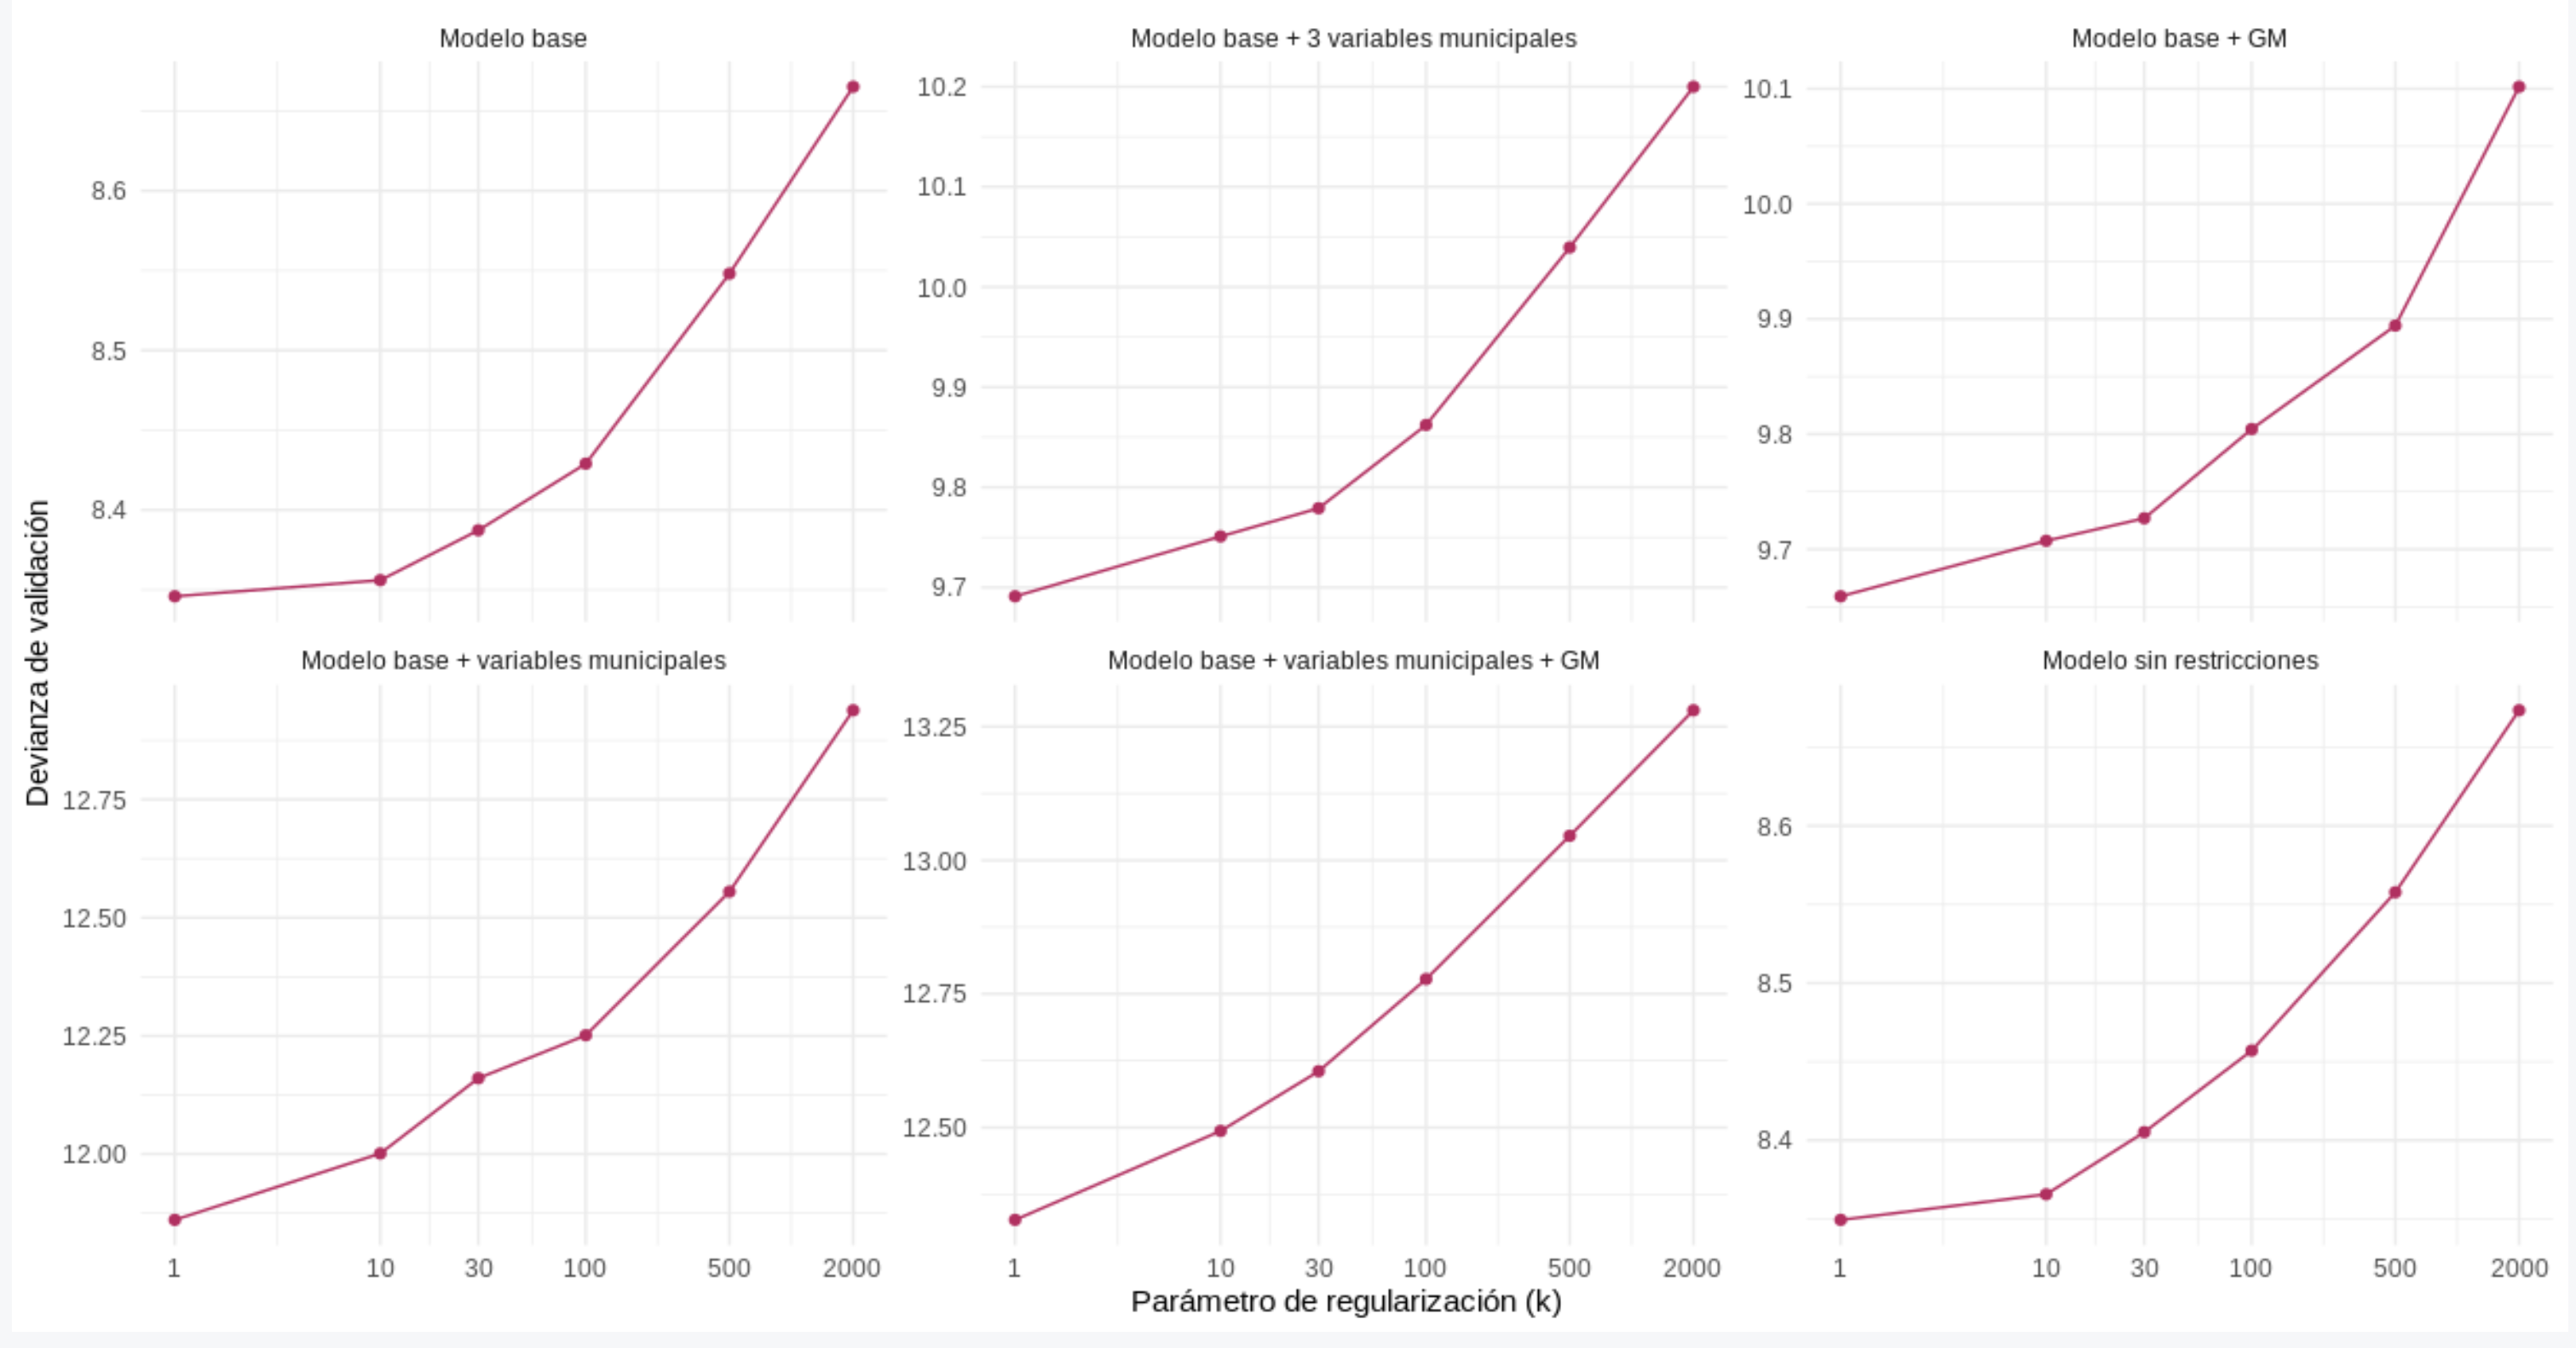
\includegraphics[height=14cm, width=18cm]{devianza_validacion}
\end{figure}
\section*{Comparando distintos conjuntos de variables}
Una vez que escogimos la mejor estructura posible dado un conjunto de variables, es necesario construir el clasificador que mencionamos anteriormente. Necesitamos entonces hacer inferencia probabilística para obtener un estadístico que nos ayude con la tarea de clasificación.
\par
\noindent
Existen varios algoritmos para hacer inferencia en Redes Bayesianas. Nosotros consideramos dos: \textit{logic sampling} -parte de la familia de técnicas de muestreo por importancia- y \textit{belief propagation}, un algoritmo de paso de mensaje. La ventaja del segundo sobre el primero es que permite el cálculo de las distribuciones marginales de manera más eficiente. Además, las técnicas de muestreo por importancia pueden llevar a descartar buena parte de los elementos de la muestra, resultando así en un tiempo mayor de convergencia. Sin embargo, los algoritmos de muestreo por importancia que están implementados en R tienen menos carga de dependencias, lo cual puede resultar útil en la implementación como explicaremos más adelante.\\
Una vez que calculamos la distribución posterior de las variables ''verdaderas'' dadas las respuestas al cuestionario, podemos hacer una comparación simple y construir un estadístico que podamos interpretar como la probabilidad de tener algún incorrecto. Para esto, lo que hicimos fue restar las probabilidades de las respuestas (codificadas como variables binarias) y sumar esas diferencias. En la siguiente figura podemos observar la distribución de este estadístico, según el verdadero estado de reportaje en el cuestionario.
\begin{figure}[H]
    \caption{Suma de probabilidades según la distribución a posteriori}
    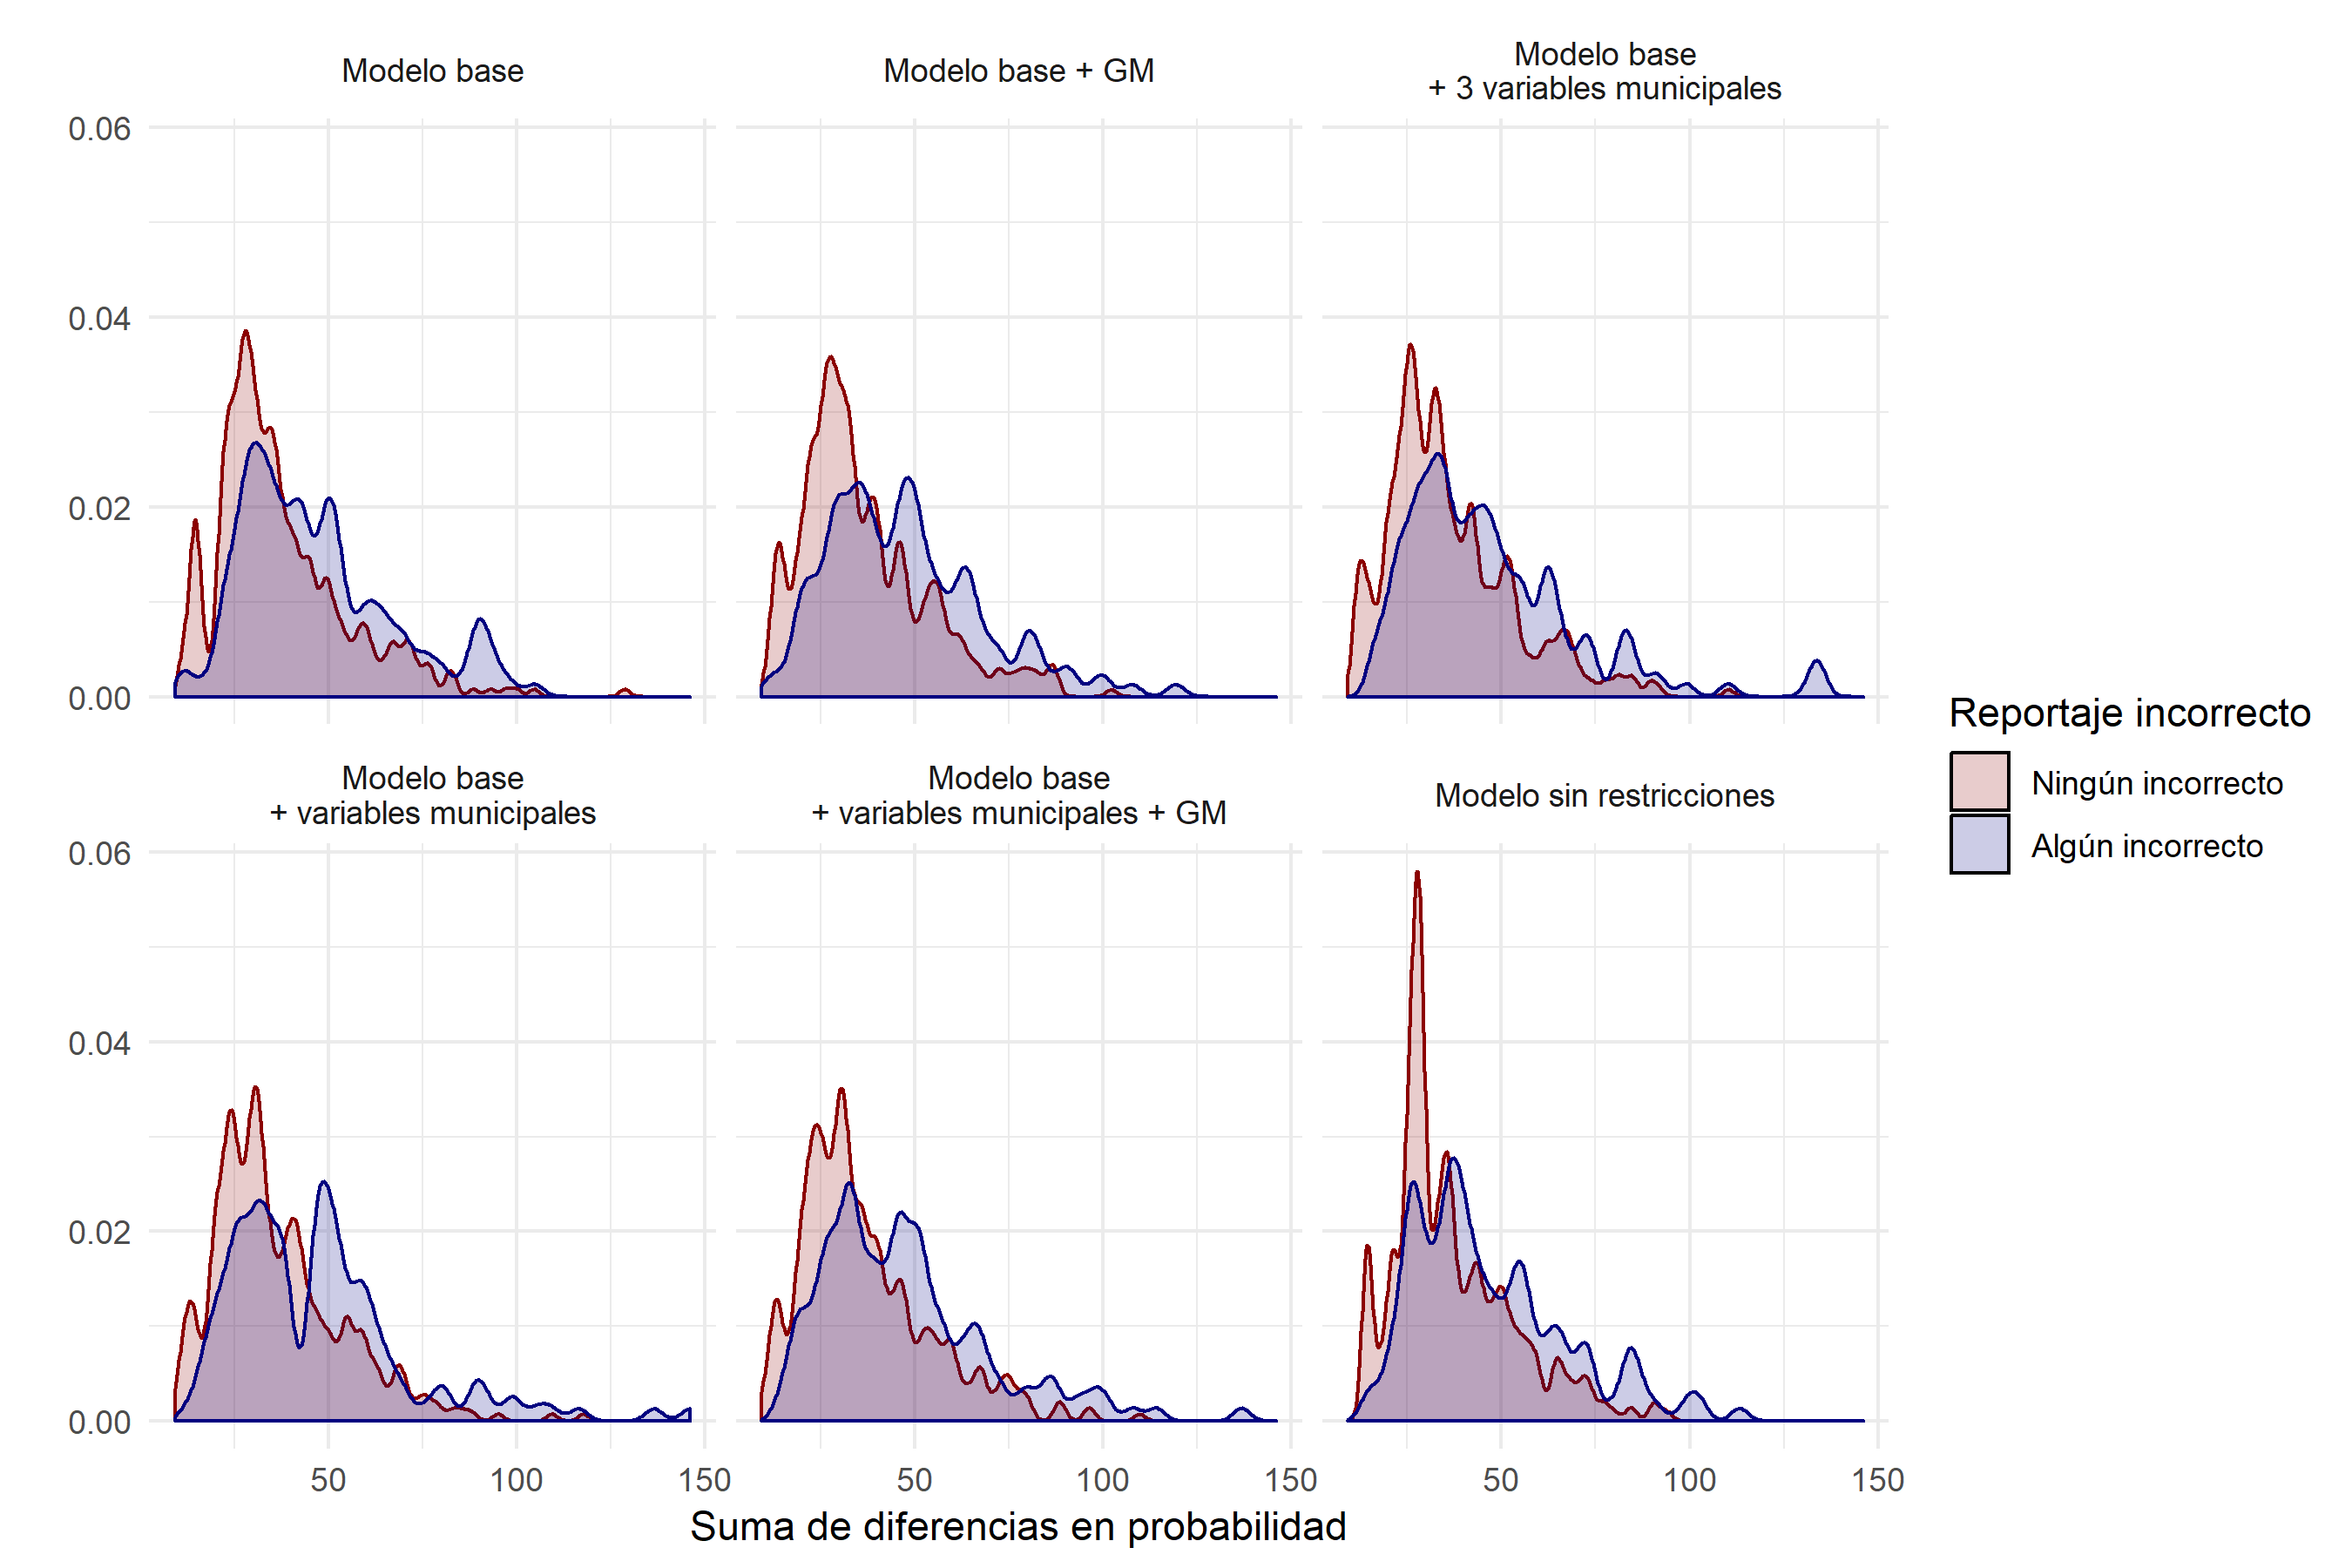
\includegraphics[width=18cm, height=12cm]{suma_probabilidades}
    {\footnotesize{Comparando las distribuciones que induce cada modelo, notemos que si bien las que tienen algún error están más sesgadas a la derecha, en general no parece fácil establecer las diferencias entre estas y las distribuciones sin error. Esto implica que necesitamos explorar más opciones para construir un mejor clasificador.}}
\end{figure}
\par
\noindent
Una vez obtenida la suma, comparamos varios puntos de corte para construir un clasificador binario, y evaluamos el clasificador utilizando el área bajo la curva ROC. La curva ROC (Receiver Operating Characteristic, por su origen naval) es una herramienta para evaluar la capacidad de un clasificador binario de discriminar conforme va variando el umbral de clasificación. Esta curva resulta de graficar la Tasa de Falsos Positivos (TFP) en el eje x, y la tasa de verdaderos positivos (TVP) en el eje Y. Estas dos métricas se definen como sigue:
\begin{align*}
    TFP := \frac{FP}{N} \\
    TVP := \frac{VP}{P}
\end{align*}
Donde $(F,V)$ son Falso y Verdadero, y $(N,P)$ son Negativo y Positivo, respectivamente. Cabe mencionar que a la TVP comúnmente se le llama \textit{sensitividad}, y que la TFP puede reescribirse como $1-TVN$, donde $TVN$ también es conocida como \textit{especificidad}. Ambas métricas son relativamente estándar en el campo de la ciencia de datos, y compararlas gráficamente tiene la intención de tomar en cuenta el intercambio que se hace entre falsos positivos y falsos negativos en la construcción de un clasificador.
\par
\noindent
\begin{figure}[H]
    \caption{Curva ROC}
    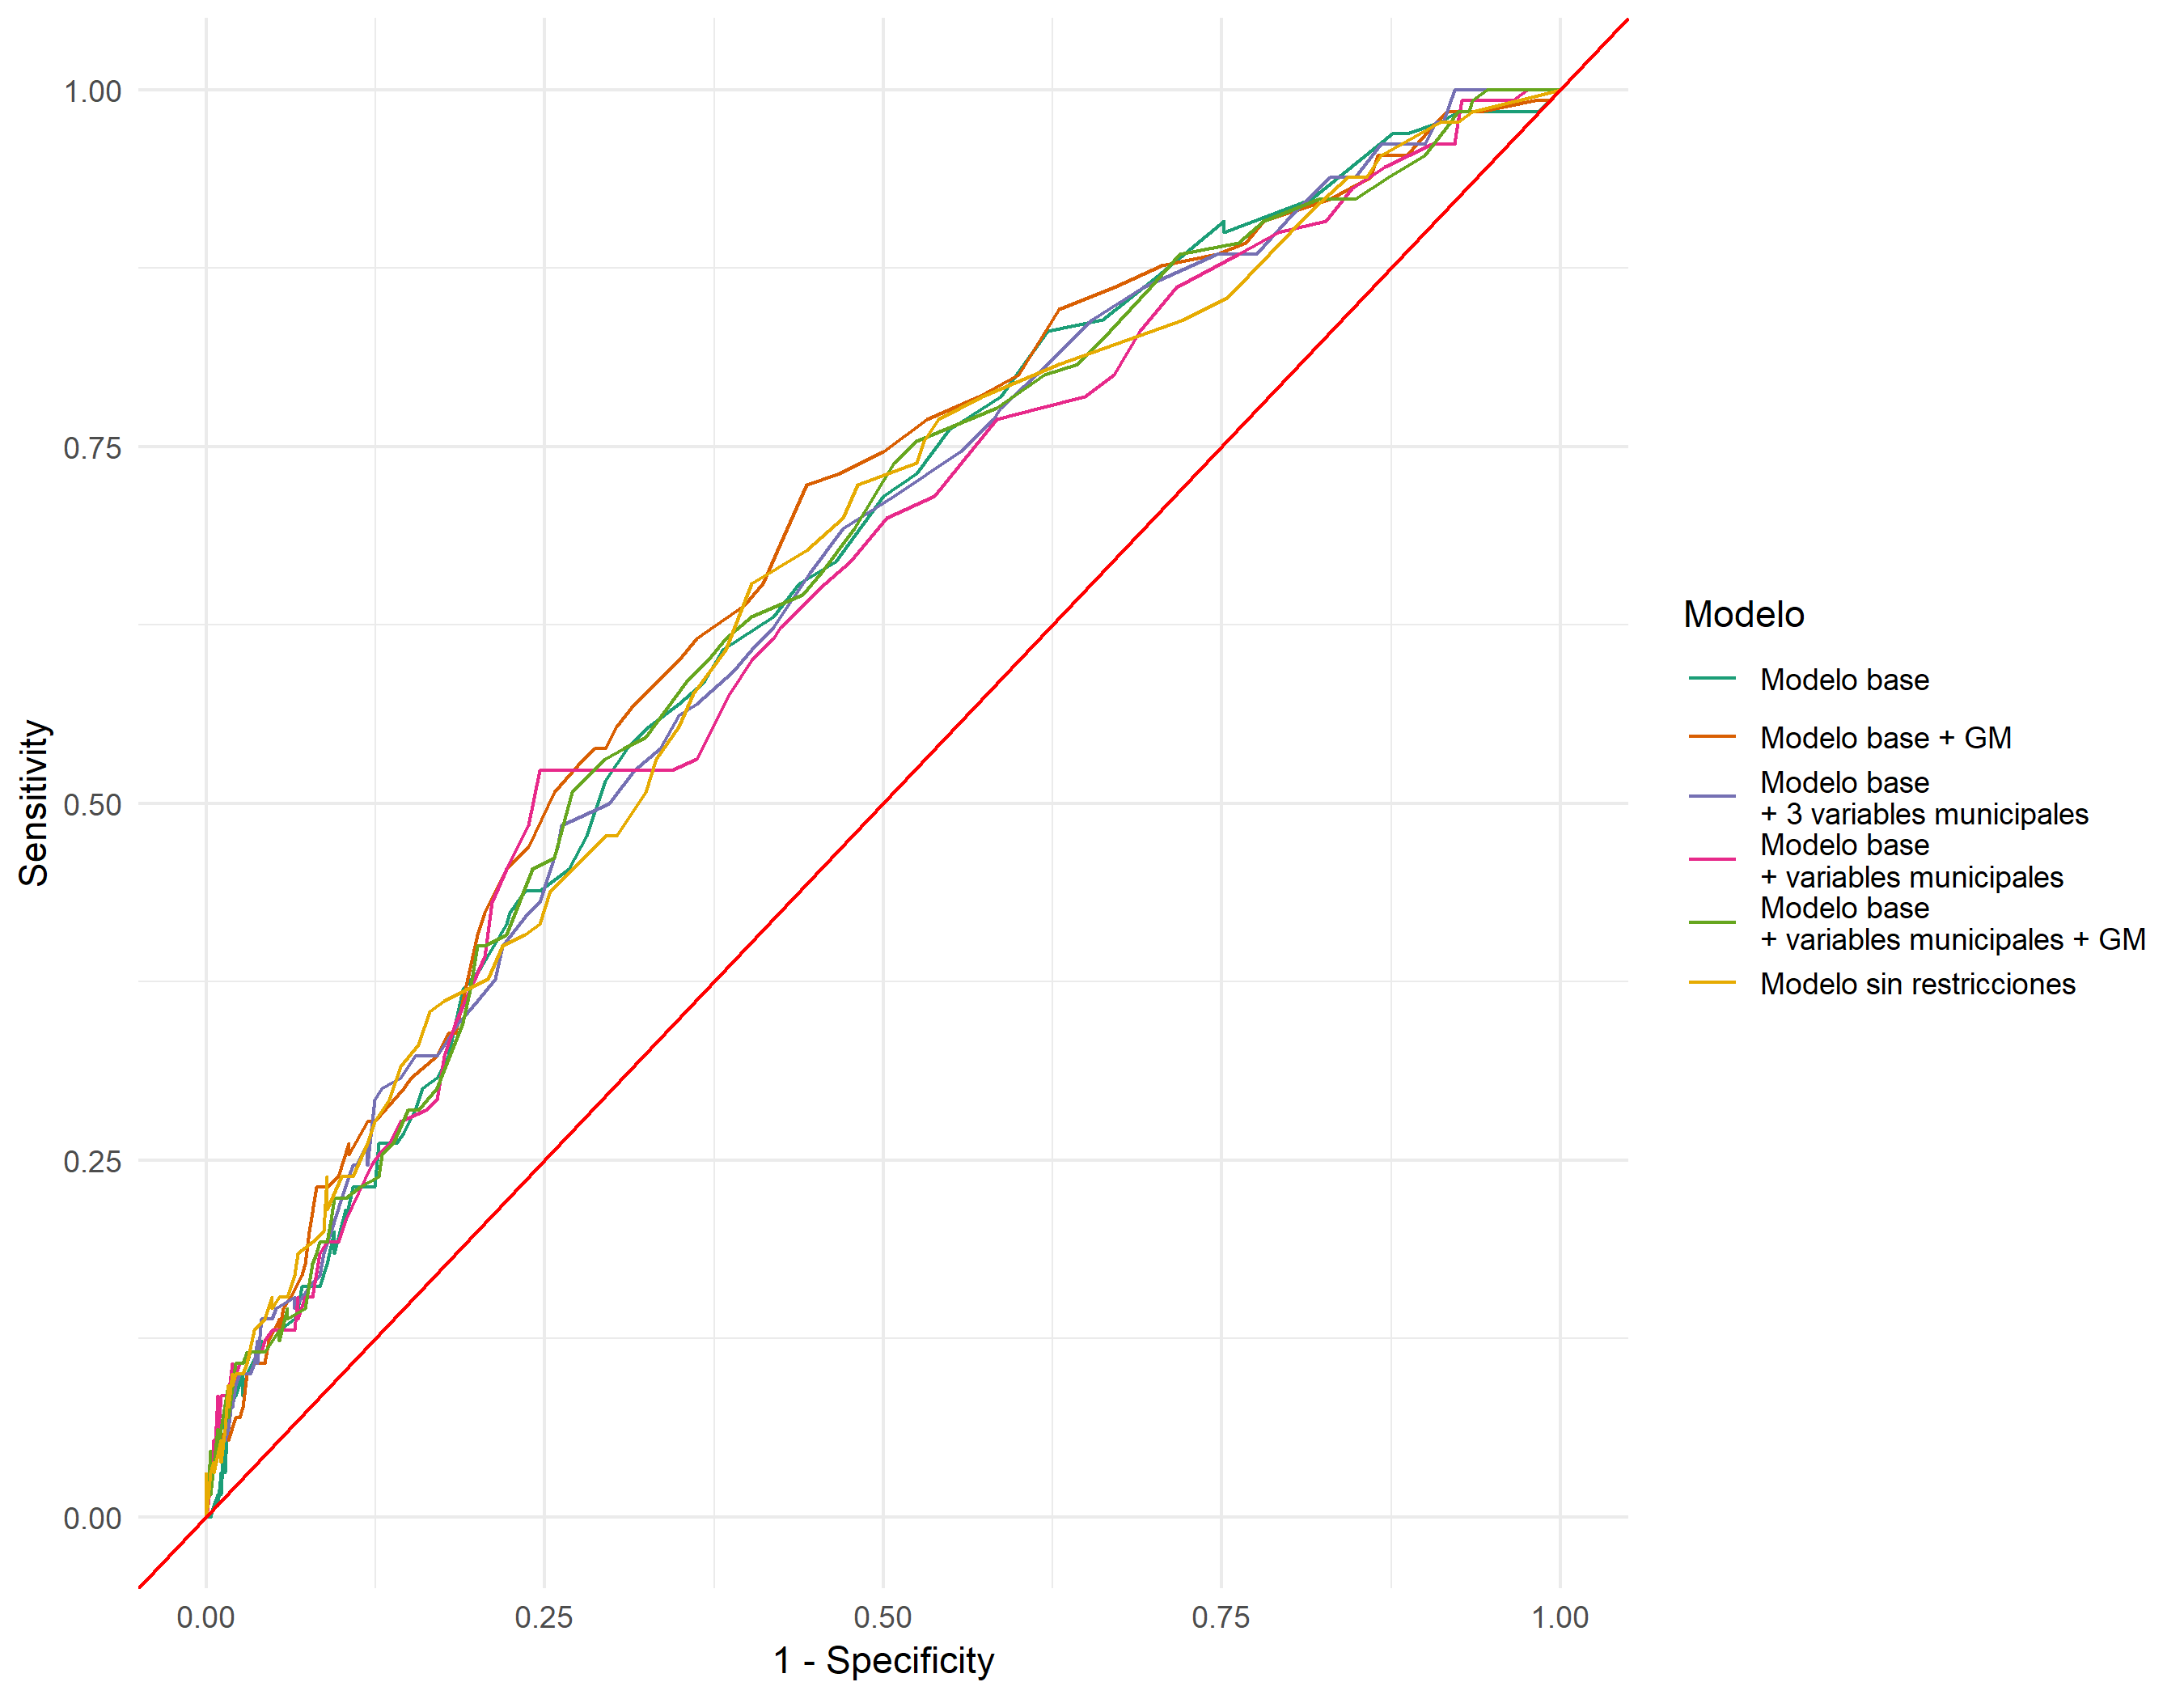
\includegraphics[height=14cm, width=18cm]{results_roc}
\end{figure}
Intuitivamente, la curva ROC de un clasificador perfecto sería una $L$ reflejada sobre el eje horizontal, y la curva ROC de un clasificador construido tirando una moneda sería la línea roja $y=x$.
\par
\noindent
Ahora, para poder evaluar la efectividad general de cada clasificador, tomando en cuenta todos los puntos de corte, se utiliza generalmente el área bajo la curva ROC (AUC, por sus siglas en inglés). En este caso utilizamos la Regla del Trapecio para calcular el AUC a partir de la colección de puntos obtenida.
\begin{figure}[H]
    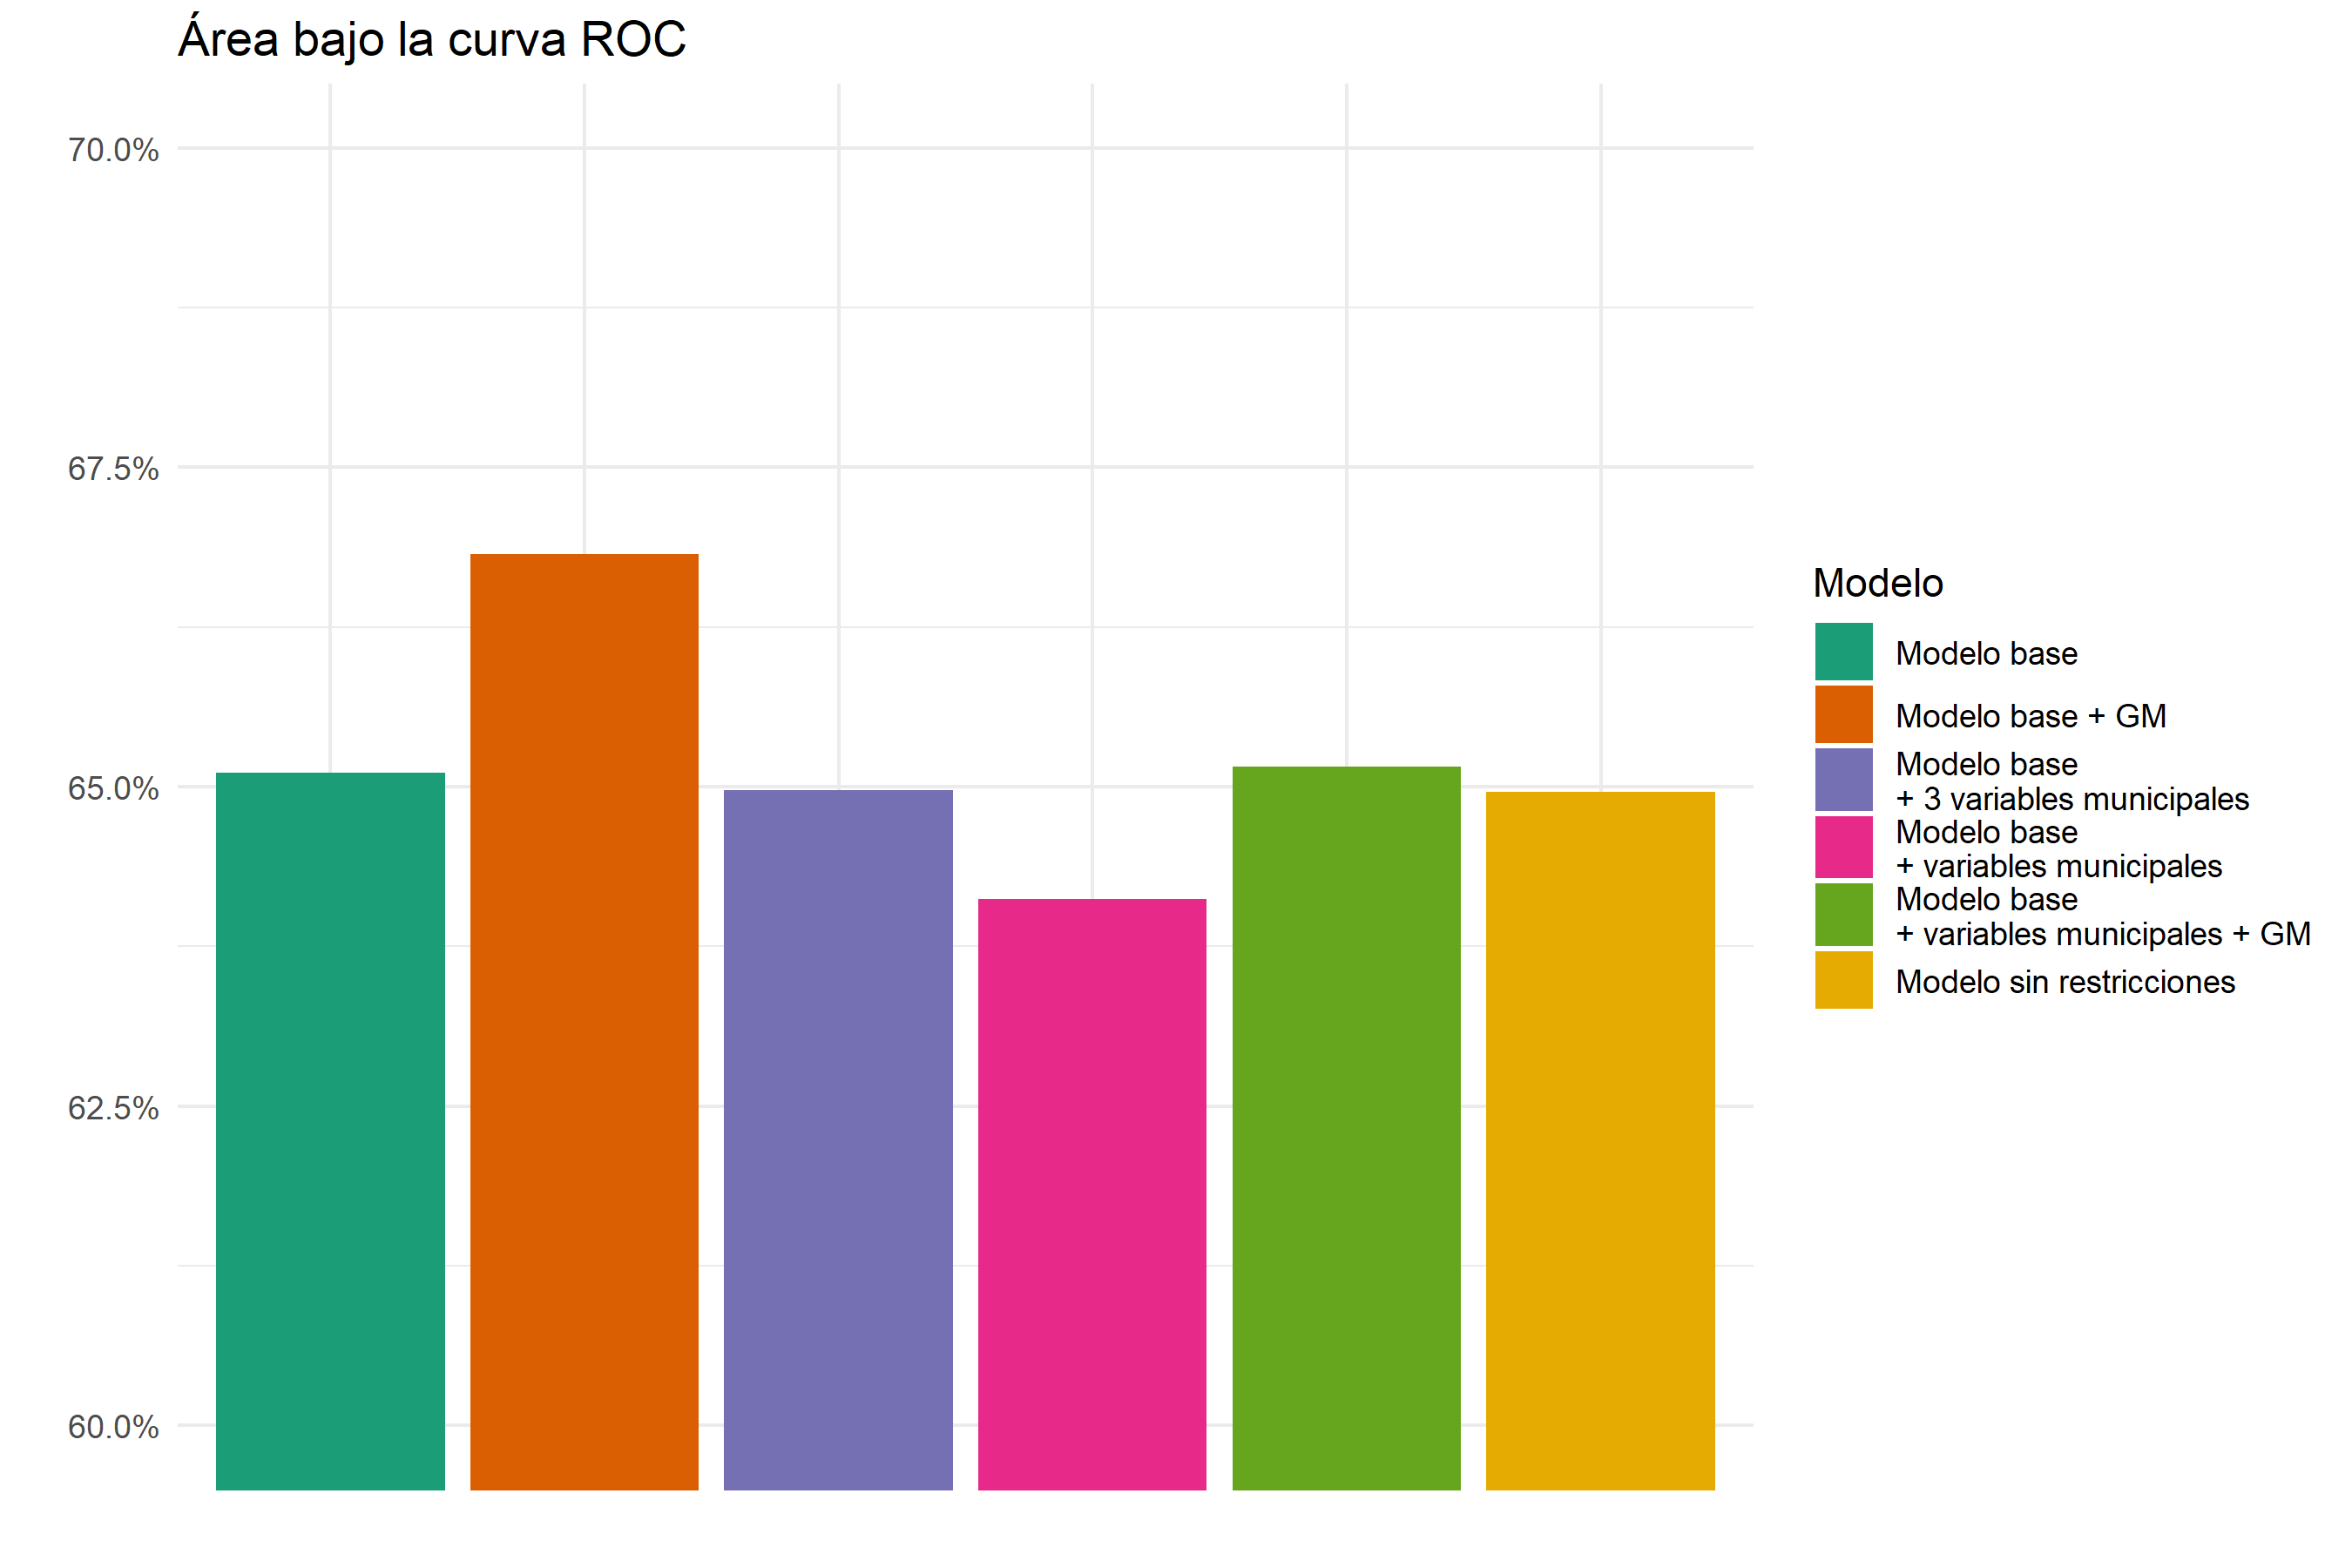
\includegraphics[height=14cm, width=18cm]{results_auc}
    \footnotesize{Notemos que hemos limitado el rango del eje y para efectos de comparabilidad entre modelos, pero el resultado del AUC varía relativamente poco entre ellos.}
\end{figure}
Los resultados indican que el Modelo Base con grado de marginación induce un clasificador ligeramente mejor que los otros. Además, si comparamos las estructuras de los modelos, el grado de marginación sí parece estar resumiendo gran parte de la información que tienen el resto de las variables. Decidimos utilizar este modelo para la implementación del piloto, pero tenemos una serie de recomendaciones para seguir esta exploración:
\begin{itemize}
    \item Explorar más conjuntos de variables a nivel municipal, y otro tipo de discretizaciones.
    \item Reentrenar el modelo con los resultados del piloto. Intuitivamente, tiene sentido pensar que las tasas de reportaje incorrecto sean mayores en programas que no hacen verificaciones domiciliarias a todos sus cuestionarios.
    \item Explorar los patrones de sub y sobrerreporte obtenidos del piloto, buscando reducir la dimensionalidad del problema.
\end{itemize}
